\documentclass[11pt,english]{article}

\usepackage[english]{babel}
\usepackage{enumitem}
\usepackage{fancyhdr}
\usepackage{graphicx}
\usepackage{lastpage}

\pagestyle{fancy}

\graphicspath{{assets/}}

\lfoot{}
\cfoot{\today}
\rfoot{\thepage/\pageref{LastPage}}

\newcommand*{\Frontpage}{\begingroup
  \hbox{%
    \hspace*{0.2\textwidth}
    \rule{1pt}{\textheight}
    \hspace*{0.05\textwidth}
    \parbox[b]{0.75\textwidth}{%
      {\noindent\Huge\bfseries IDPRI}\\[2\baselineskip] % Title
      {\large \textit{Huiswerkopdrachten}}\\[4\baselineskip] % Tagline or further description
      {\Large \textsc{\\
          Patrick Spek, 2099745 \\
          Roy, 2097591 \\
        }}
      \vspace{0.5\textheight} % Whitespace between the title block and the publisher
    }
  }
\endgroup}

\renewcommand{\footrulewidth}{0.4pt}

\begin{document}
  \thispagestyle{empty}
  \Frontpage
  \newpage

  \tableofcontents
  \newpage

  \section{Opdracht 1}
  \subsection{Taakgeschiktheid}
  Duidelijke, simpele layout voor beginnende gebruikers. Uitgebreide hotkeys
  voor frequente gebruikers.

  \subsection{Consistentie}
  Er wordt gebruik gemaakt van een Bootstrap thema zodat de applicatie er overal
  hetzelfde uitziet.

  \subsection{Bestuurbaarheid}
  De buttons die een gewenste resultaat bieden zijn duidelijk te vinden. Buttons
  voor andere opties zijn beschikbaar, maar wel ``grayed-out'' zodat ze niet in
  de weg zitten voor het normale gebruik.

  \subsection{Herkenbaarheid}
  Er worden standaard icons gebruikt die iedereen kan herkennen zodat de acties
  herkenbaar zijn aan een simpel icoontje.

  \subsection{Terugkoppeling}
  Toasts geven aan wanneer een bepaalde actie is uitgevoerd zodat de gebruiker
  confirmatie heeft dat het gelukt is. Verder is er een spinner zichtbaar
  wanneer er nog data ingeladen wordt.

  \subsection{Eenvoud}
  Er worden geen onnodige buttons toegevoegd die het systeem moeilijker maken
  dan het is.

  \subsection{Aantrekkelijkheid}
  Er wordt gebruik gemaakt van mooie (maar duidelijk leesbare) fonts tegen een gekleurde achtergrond. 

  \subsection{Tolerantie}
  "Confirmation-buttons" vragen om bevestiging voor invloedrijke acties.

  \subsection{Flexibiliteit}
  Zoals ook opgemerkt bij taakgeschiktheid, wordt er een simpele layout gebruikt
  voor beginnende gebruikers. Geavanceerde gebruikers kunnen hun workflow
  versnellen door middel van hotkeys.

  \section{Opdracht 2}
  \subsection{Login}
  \begin{center}
    \makebox[\textwidth]{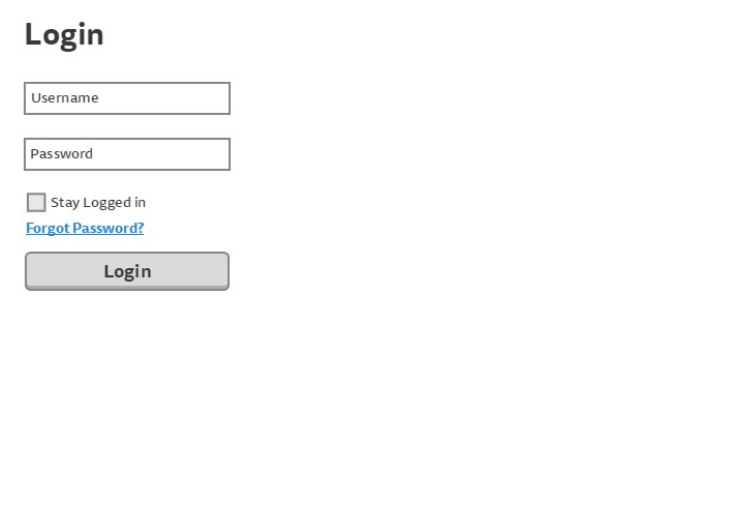
\includegraphics[width=\linewidth]{wf-login}}
  \end{center}

  \subsection{Welcome}
  \begin{center}
    \makebox[\textwidth]{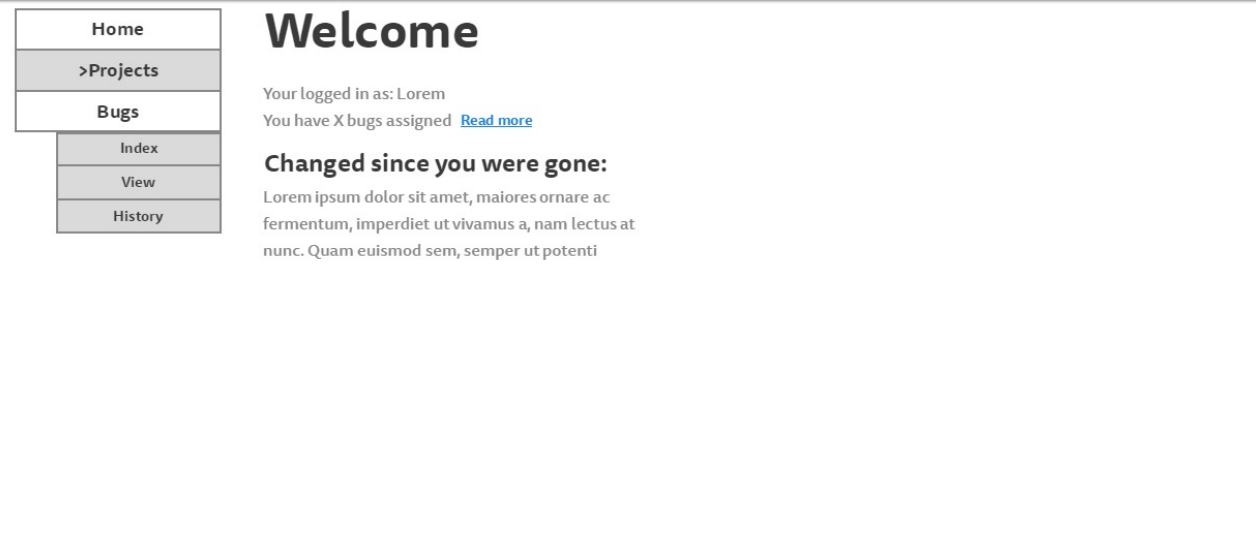
\includegraphics[width=\linewidth]{wf-welcome}}
  \end{center}

  \subsection{Projects}
  \begin{center}
    \makebox[\textwidth]{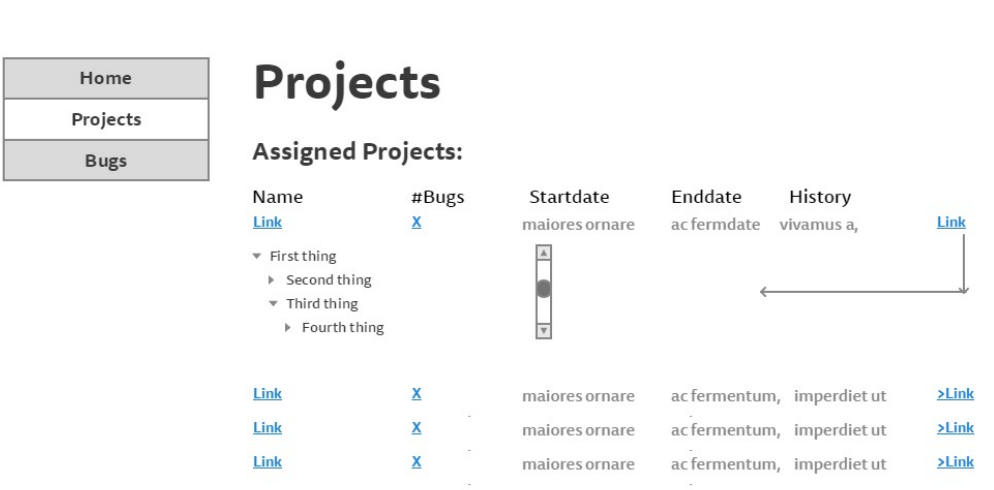
\includegraphics[width=\linewidth]{wf-projects}}
  \end{center}

  \subsection{Bug index}
  \begin{center}
    \makebox[\textwidth]{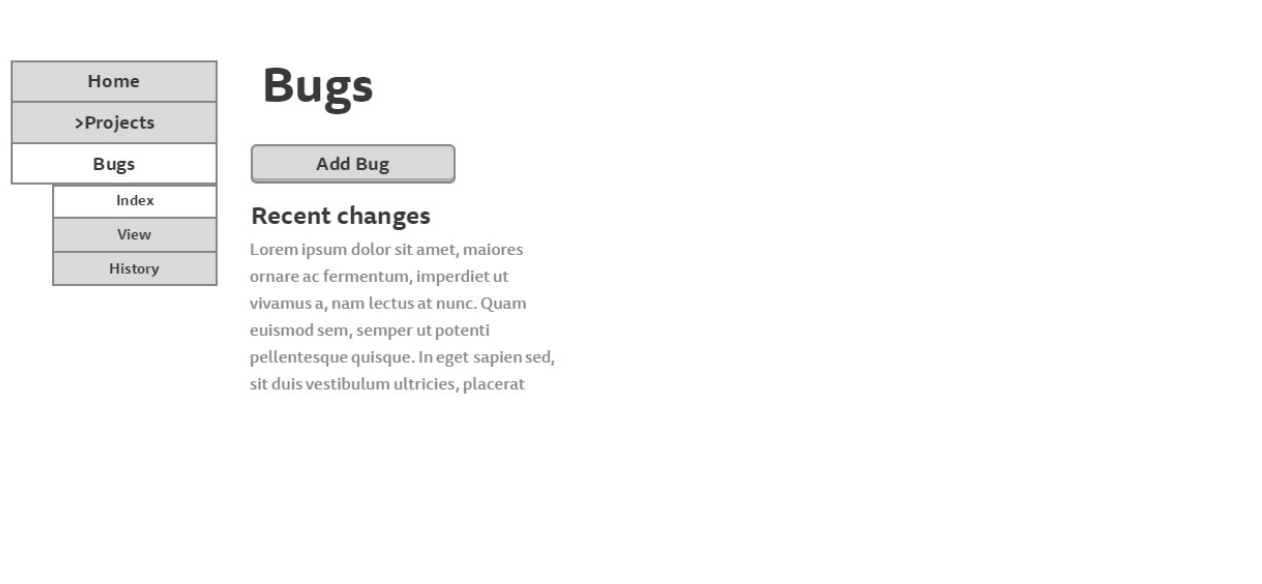
\includegraphics[width=\linewidth]{wf-bugsindex}}
  \end{center}

  \subsection{Bug view}
  \begin{center}
    \makebox[\textwidth]{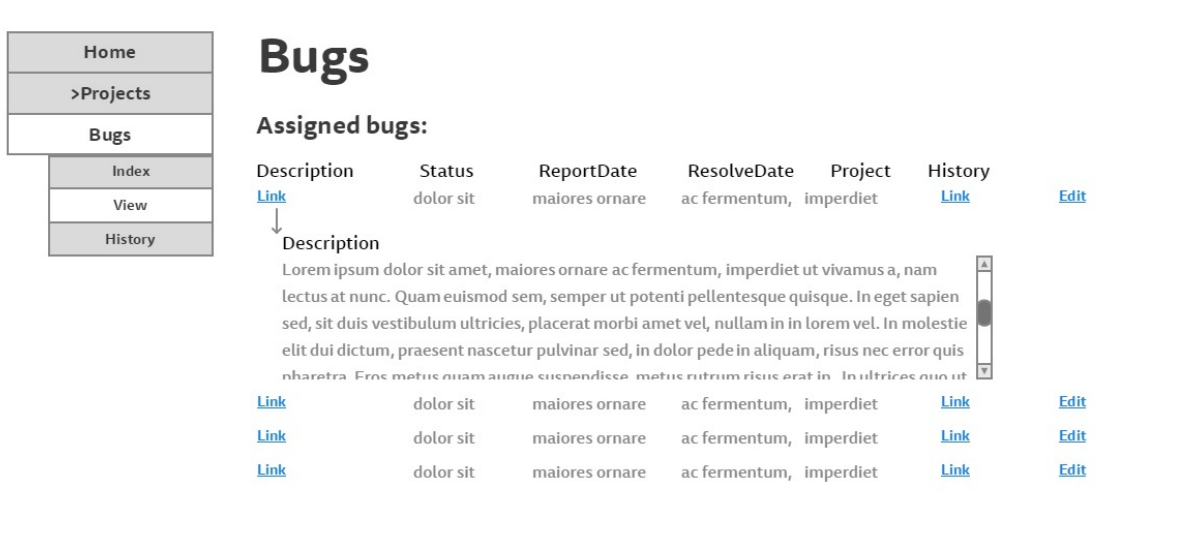
\includegraphics[width=\linewidth]{wf-bugs}}
  \end{center}

  \subsection{Assigned bugs}
  \begin{center}
    \makebox[\textwidth]{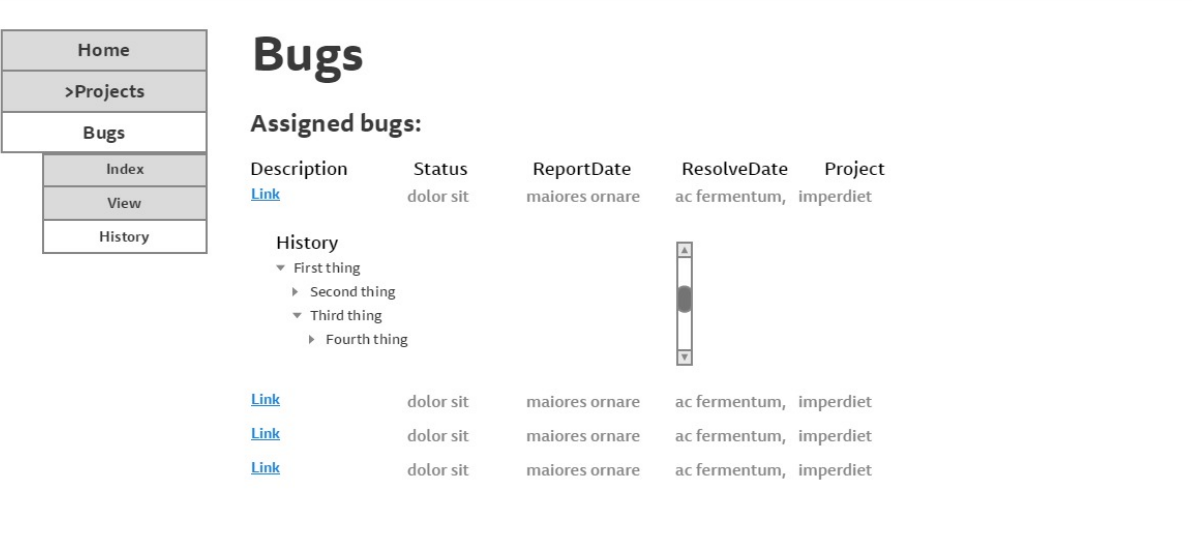
\includegraphics[width=\linewidth]{wf-assignedbugs}}
  \end{center}
\end{document}

